%!TEX root = ../template.tex
%%%%%%%%%%%%%%%%%%%%%%%%%%%%%%%%%%%%%%%%%%%%%%%%%%%%%%%%%%%%%%%%%%%%
%% chapter5_PrototypingPerf.tex
%% NOVA thesis document file
%%
%% Chapter with the Prototyping and Performance Evaluation Results part
%%%%%%%%%%%%%%%%%%%%%%%%%%%%%%%%%%%%%%%%%%%%%%%%%%%%%%%%%%%%%%%%%%%%

\typeout{NT FILE chapter5_PrototypingPerf.tex}

\chapter{Prototyping and Performance Evaluation Results}\label{cha:chapter5_PrototypingPerf}

%So neste capitulo e que se deve descrever a operacao do circuito.
Upon completion of the circuit design phase, the next step starts to dictate the physical shape of the prototype.

\section{PCB Layout}\label{sec:5_PCBlayout} % se calhar tiro "Design"
%provavelmente este capitulo deve ficar no final do Chapter 4, porque layout também é hardware design

Once every component symbol in the schematics is correctly referenced and the electrical rules check reports no errors nor warnings, KiCad provides a footprint assignment tool, to attribute the desired footprints to the project's parts. Since the new beRTK\textsuperscript{\textregistered} circuit is based around fourteen main ICs and modules, selecting the correct footprints for each of these was the starting point for the layout phase. For that, datasheets for ICs and modules usually feature a section dedicated to presenting the recommended footprint for their component. This facilitates designers' work, as KiCad already provides a vast list of footprint libraries with many footprints to choose from, and therefore the attribution boiled down to a simple matter of finding the correct matches, referring to the datasheets. Figure~\ref{fig:footprint_AP64501} shows the recommended solder pad pitch and dimensions for the AP64501 buck converter addressed in Section~\ref{sec:3214_AP64501}, an example of what is taken as reference when assigning footprints.

% meter aqui footprint LTC4012 - datasheet
\begin{figure}[h]
	\centering
	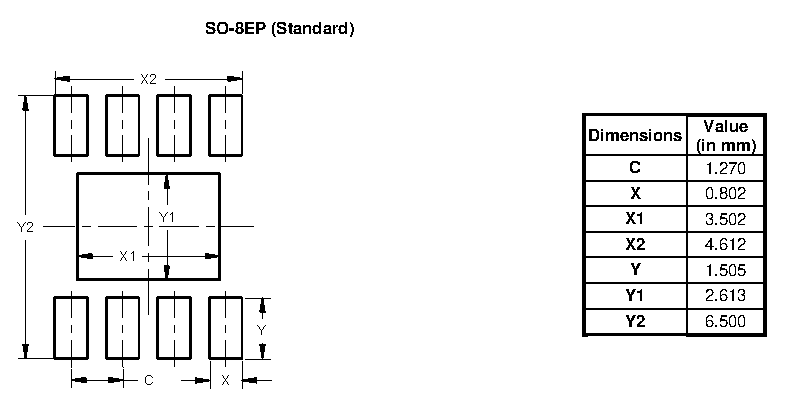
\includegraphics[width=0.7\textwidth]{Chapters/Figures/chapter5/footprint_AP64501.pdf}
	\caption{Recommended solder pad pitch and dimensions for the AP64501 synchronous buck converter~\cite{AP64501}.}
	\label{fig:footprint_AP64501}
\end{figure}

For the ICs and modules whose footprints are not provided by default by the software, internet research was conducted in order to find them -- \url{https://www.snapeda.com/} and \url{https://pt.mouser.com/} were the two websites accessed for such purpose, since these are known to provide trustworthy footprints.

Regarding resistors, unless otherwise stated, all should have a 0805 \gls{SMD} package footprint and a tolerance of 5\%. The standard 0805 package size measures $0.08 \times 0.05$ inches (length $\times$ width), which corresponds, in the metric system, to a 2012 package size, at $2.0 \times 1.25$ millimetres (length $\times$ width).
Capacitors should also have a 0805 SMD package footprint and be rated for 50V, unless otherwise stated.
As for the remaining components, i.e. MOSFETs, diodes, inductors, ferrites, crystal and connectors, their footprint depends on the application.
Datasheets of ICs and modules usually refer the characteristics and/or models to use in a typical implementation.

To effectively design the board's layout, KiCad provides a PCB editor that directly places the assigned footprints in single editing window. These footprints must then be placed according to their respective component's location in the schematic, in the most efficient way possible among the other components. The PCB editor also displays white lines (known as ``ratsnest lines'') that connect different components' pads to each other, just as defined by the schematic design. This helps in the subsequent routing process (i.e. effectively connecting every component with tracks and/or vias). Figure~\ref{fig:ratsnest} shows an early version of the layout for the external power supply region of the system, which is connected to the LTC4012 and to the external power voltage reference (top left area of the schematic of Figure~\ref{fig:LTC4012_circuit}).

\begin{figure}[h]
	\centering
	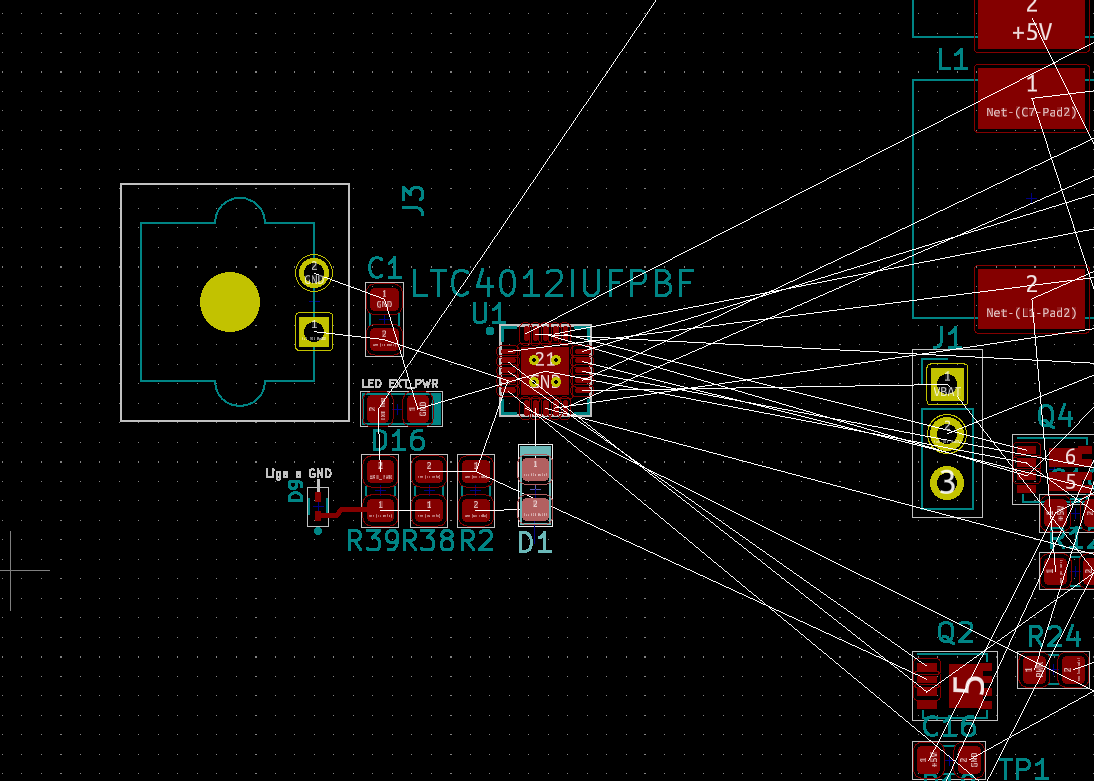
\includegraphics[width=1.0\textwidth]{Chapters/Figures/chapter5/ratsnest.png}
	\caption{Unconnected footprints for the external power supply region of the system (early version).}
	\label{fig:ratsnest}
\end{figure}

%parei aqui:
%0. falar do placement estar concluido:
%   dizer que é importante o cristal estar mais perto possivel do LAN, porque o routing desta parte do circuito é critica;
%   importante as USB downstream ports estarem o mais perto possivel do LAN
%   ver se me lembro de mais regras...
%   definiu-se um limite experimental para a placa ($100 \times 70$ mm (length $\times$ width)) e acabou por se aumentar para $129 \times 90$ mm (length $\times$ width).

%   depois começa o routing:
%1. falar das minimum design rules da eurocircuits
%2. falar das minimum design rules que eu usei, que sao um pouco diferentes
%3. dizer a thickness da placa, 4 layers -- 2 signal, 2 pwr -- mostrar a janela do kicad
%4. falar das thickness das tracks de power, de signal, tamanho das vias de power, de signal. clearance
%4.1 definiram se os signal, power, GND planes.
%5. dizer que o primeiro routing que se fez foi o mais critico --  USB e HDMI -- que tambem têm tracks com tamanhos especificos -- falar e mostrar as contas desses tamanhos (impedance matching).
%4. importante que as power tracks passem pelos capacitors primeiro e so depois vao para o power plane (5V), para que os condensadores possam cumprir devidamente o seu propósito de bypassing.



-- $20 \mu$F ceramic capacitors were chosen for both the power inputs and power output of the LTC4012. 

-- As mentioned before, the top and bottom power FETs Q2 and Q9, along with inductor L1 are vital to the PWM control architecture. These components are part of the sub-circuit that starts from the +15VDC source of power and passes across FET Q1 (connected to pin INFET), sense resistor R3, 
This sub-circuit forms the ``power supply rail'', and upon layout design of the circuit from Figure~\ref{fig:LTC4012_circuit}, this section must bear a track width large enough to withstand large values of currents or any other phenomena that may occur (e.g. voltage/current spikes). The needed track width can be calculated through the following expression:

XBee: Digi XBee 3 RF Module Hardware Reference Manual
We design XBee 3 RF Modules to be self-sufficient and have minimal sensitivity to nearby processors,
crystals or other printed circuit board (PCB) components. Keep power and ground traces thicker than
signal traces and make sure that they are able to comfortably support the maximum current
specifications. There are no other special PCB design considerations to integrate XBee 3 RF Modules,
with the exception of antennas.

\section{PCB Manufacture}\label{sec:51_PCBmanufacture}

\section{Component Acquisition}\label{sec:52_ComponentAcquisition}

%ate agora foram os unicos MOSFETs que nao disse o nome:

%como nao foi relevante, ate agora ainda nao disse que MOSFETs selecionei para o power switch: Q4 e Q5.
%Q3, Q10, Q6, Q8 -- BQ29209
%PMEG2010ER - GNSS module

%LTC4012:
It should be noted that, for the top and bottom FET selection stage, the Si7212DN model suggested is a double FET in one package. The CSD17308Q3 substituting model is a single-channel FET (only one per package), and therefore two units had to be acquired -- Section~\ref{sec:3211_LTC4012}.

% AP64501:
Recalling Section~\ref{sec:3214_AP64501}, it is stated that the closest commercially available values of 11k$\Omega$ and 2.7k$\Omega$ were selected for R10 and R13, respectively, at the prototyping phase. Following expressions (\ref{eq:R10}) and (\ref{eq:R13}), these values allow the expected $V_{ON}$ and $V_{OFF}$ values.
    % inductor L2:
    Meter Eq. 9 do datasheet do AP64501;
    
    Peak current determines the required saturation current rating, which influences the size of the inductor. Saturating the inductor decreases the converter efficiency while increasing the temperatures of the inductor and the internal power MOSFETs. Therefore, choosing an inductor with the appropriate saturation current rating is important. 
    It is recommended by \cite{AP64501} the selection of an inductor value between $1 \mu$H to $10 \mu$H, and therefore, taking into account the values presented in Table~\ref{tab:AP64501_recommended_values}, an inductor of $3.6 \mu$H was selected. It is also advised to select an indcutor with a DC current rating of at least 35\% higher than the maximum 5A load current of the AP64501, which corresponds to 6.75A.
    For highest efficiency, the inductor's DC resistance should be less than 10mOhm. Use a larger inductance for improved efficiency under light load conditions.


% CM4:
    At just 40mm $\times$ 55mm and 4.7mm deep, the form factor of the CM4 is one of its biggest advantages, since it allows designers to fit it in almost all designs.

    %HDMI routing:
    HDMI signals should be routed as 100Ohm differential pairs. Each signal within a pair should ideally be matched to better than 0.15mm. Pairs don't typically need any extra matching, as they only have to be matched to 25mm.

    %USB routing:
    The differential pair should be routed as a 90Ohm differential pair. The length of the P/N signals should ideally be matched to better than 0.15mm.

    6. The port is capable of being used as a true USB On-The-Go (OTG) port. While there is no official documentation, some users have had success making this work. The USB\_OTG\_ID pin is used to select between USB host and device that is typically wired to the ID pin of a Micro USB connector. To use this functionality it must be enabled in the OS. If using either as a fixed slave or fixed master, please tie the USB\_OTG\_ID pin to ground. tentei isto e nao deu.


% LAN9514:
    However, USB has the advantage of allowing hot-swapping, making it useful for mobile peripherals, including drives of various kinds. -- mesmo que digam isto ja é possivel por natureza do USB, eu ainda tentei fazer o que dizia no datahseet do LAN9514 para dar enable ao hot-swapping, mas continuou sem funcionar.

\section{Prototype Assembly}\label{sec:53_PrototypeAssembly}

\section{Functional Testing and Results}\label{sec:54_FunctionalTesting}